\documentclass[border=10pt]{standalone}
\usepackage[svgnames]{xcolor}
\usepackage{amsmath}
\usepackage{pgfplots}
\pgfplotsset{compat=newest}
\usepackage[sfdefault]{FiraSans}
\usepackage{FiraMono}
\renewcommand*\familydefault{\sfdefault}
\begin{document}
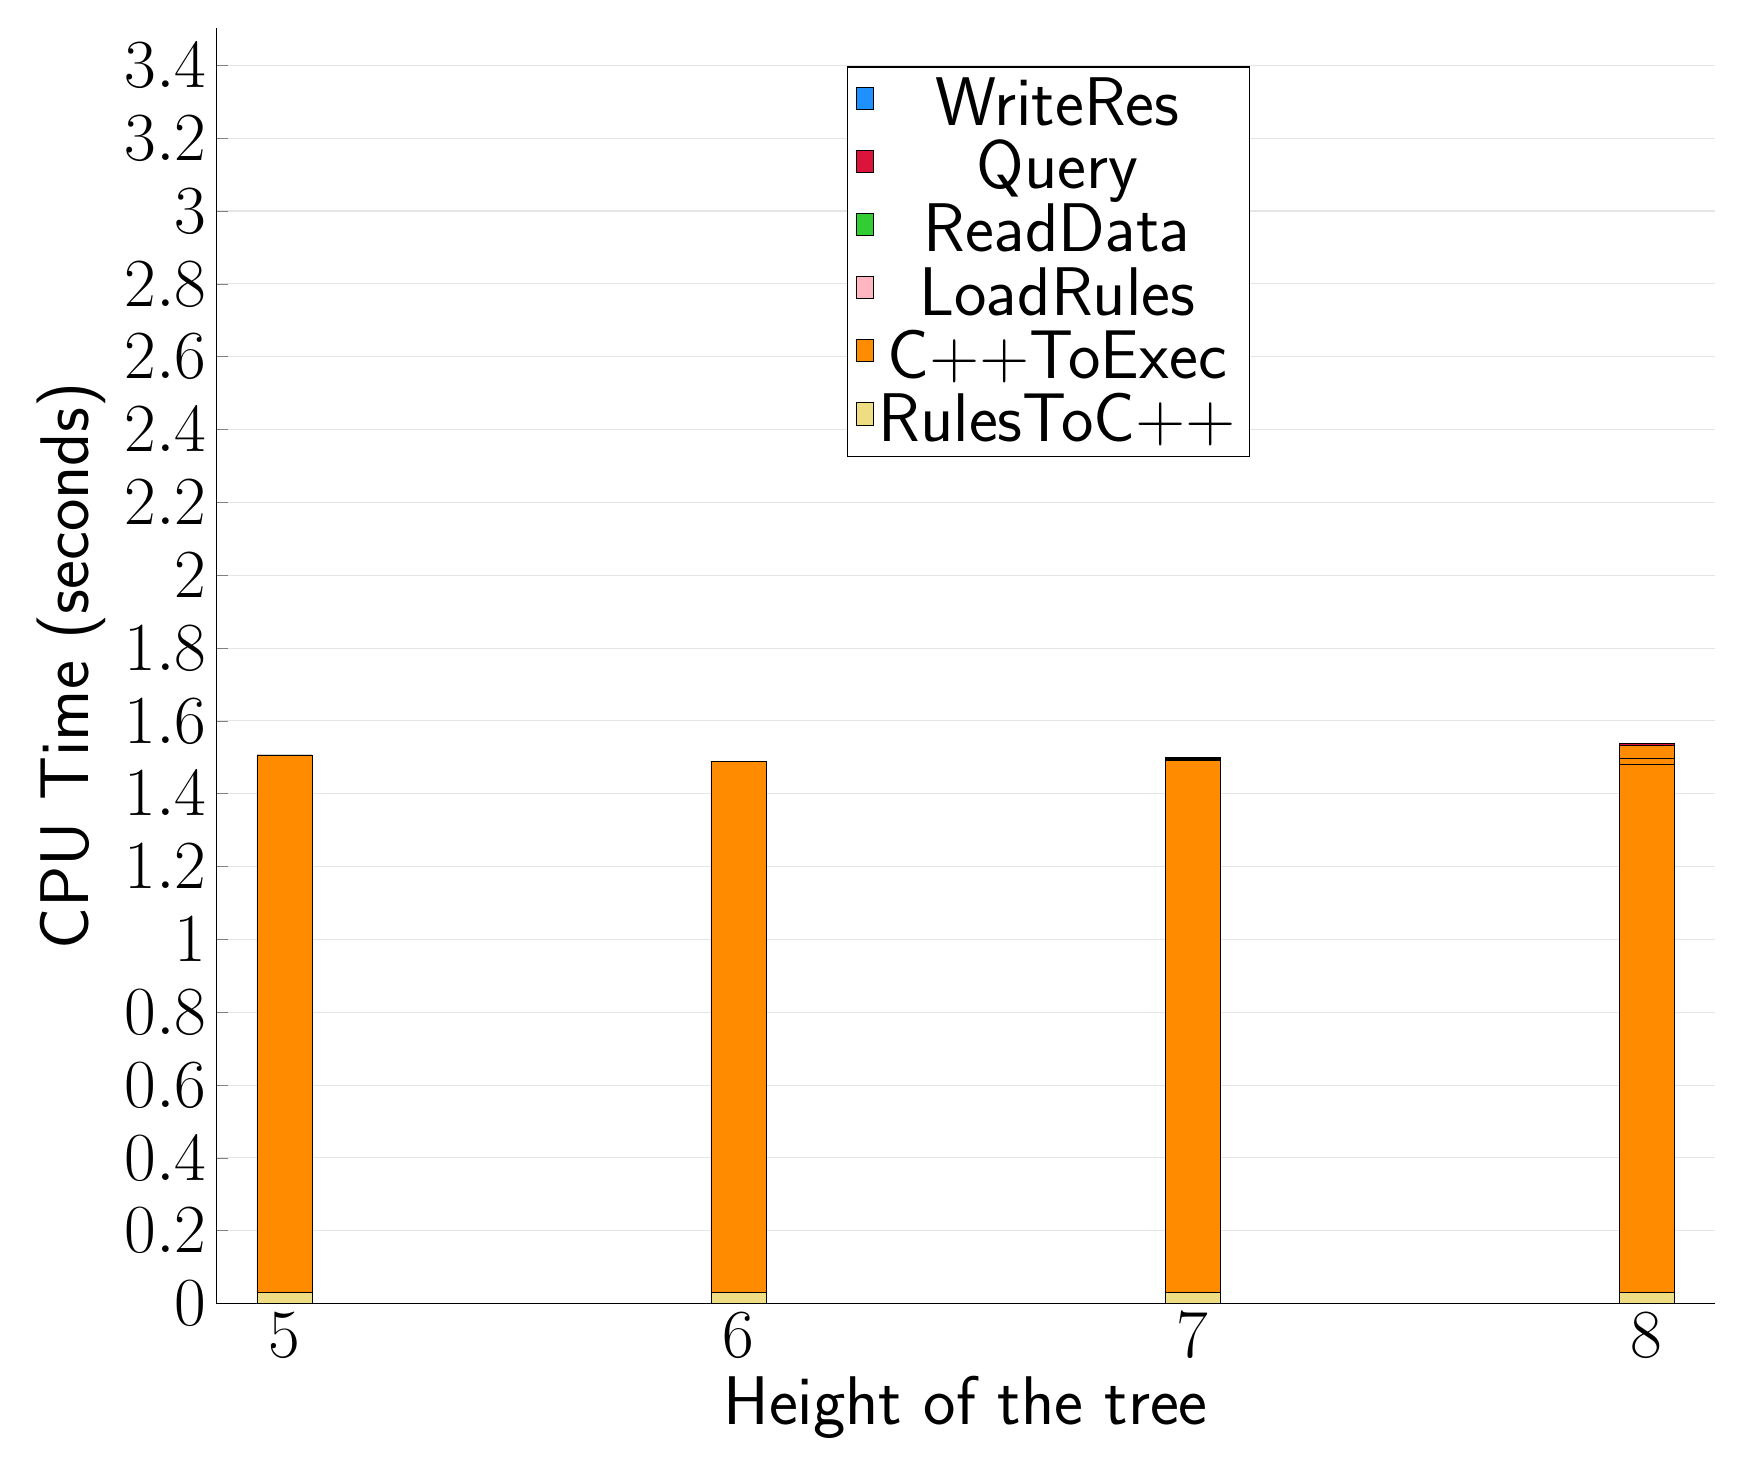
\begin{tikzpicture}
\begin{axis}[
   ybar stacked,
   width=1.7\textwidth,
   bar width=0.7cm,
   ymajorgrids, tick align=inside,
   major grid style={draw=gray!20},
   xtick=data,
   ymin=0, ymax=3.5020000000000002,
   axis x line*=bottom,
   axis y line*=left,
   enlarge x limits=0.05,
   legend style={
       at={(0.69, 0.97)},
       anchor=north east,
       legend columns=1,
       font=\Huge,
   },
   ylabel={CPU Time (seconds)},
   xlabel={Height of the tree},
   label style={font=\Huge},
   tick label style={font=\Huge},
]
\addlegendimage{fill=DodgerBlue, draw=black, line width=0.2pt}
\addlegendentry{WriteRes}
\addlegendimage{fill=Crimson, draw=black, line width=0.2pt}
\addlegendentry{Query}
\addlegendimage{fill=LimeGreen, draw=black, line width=0.2pt}
\addlegendentry{ReadData}
\addlegendimage{fill=LightPink, draw=black, line width=0.2pt}
\addlegendentry{LoadRules}
\addlegendimage{fill=DarkOrange, draw=black, line width=0.2pt}
\addlegendentry{C++ToExec}
\addlegendimage{fill=LightGoldenrod, draw=black, line width=0.2pt}
\addlegendentry{RulesToC++}
\addplot +[fill=LightGoldenrod, draw=black, line width=0.2pt] coordinates {
(5, 0.030000000000000006)
(6, 0.030000000000000006)
(7, 0.031000000000000007)
(7, 0.030000000000000006)
(7, 0.030000000000000006)
(8, 0.030000000000000006)
(8, 0.031000000000000007)
(8, 0.030000000000000006)
};
\addplot +[fill=DarkOrange, draw=black, line width=0.2pt] coordinates {
(5, 1.4760000000000002)
(6, 1.4579999999999997)
(7, 1.4659999999999997)
(7, 1.465)
(7, 1.4620000000000002)
(8, 1.5020000000000002)
(8, 1.467)
(8, 1.4509999999999996)
};
\addplot +[fill=LightPink, draw=black, line width=0.2pt] coordinates {
(5, 0.00011860000000000002)
(6, 8.8e-05)
(7, 9.92e-05)
(7, 9.96e-05)
(7, 6.82e-05)
(8, 7.439999999999999e-05)
(8, 0.0001104)
(8, 0.0001098)
};
\addplot +[fill=LimeGreen, draw=black, line width=0.2pt] coordinates {
(5, 0.0002906)
(6, 0.00040349999999999994)
(7, 0.0005455)
(7, 0.0005363)
(7, 0.0004936)
(8, 0.0007706000000000001)
(8, 0.0008191)
(8, 0.0008298000000000001)
};
\addplot +[fill=Crimson, draw=black, line width=0.2pt] coordinates {
(5, 0.0002662)
(6, 0.0008383999999999999)
(7, 0.0022268)
(7, 0.0022058999999999994)
(7, 0.0019904)
(8, 0.005409000000000001)
(8, 0.0057082)
(8, 0.0058922)
};
\addplot +[fill=DodgerBlue, draw=black, line width=0.2pt] coordinates {
(5, 0.00026849999999999997)
(6, 0.0003728)
(7, 0.0005154000000000001)
(7, 0.0005147999999999999)
(7, 0.0004741)
(8, 0.0008629999999999998)
(8, 0.0009075)
(8, 0.0009140999999999999)
};
\end{axis}
\end{tikzpicture}

\end{document}
